Die folgende Analyse untersucht die Singleton-Anfrage
\(x\perp_{\mathsf{st}}y\mid Z\). Im Mittelpunkt steht die Frage, ob und in
welcher Form größere Konditionierungsmengen die beobachtete Unabhängigkeit
und die praktische Lösbarkeit der zugehörigen QBF
\(\Phi_F^{\mathsf{st}}(\{x\},\{y\}\mid Z)\) verändern. Ein SAT-Ergebnis
belegt dabei \(x\perp_{\mathsf{st}}y\mid Z\), ein UNSAT-Ergebnis dessen
Negation. Ein TIMEOUT ist dagegen kein dritter logischer Wahrheitswert,
sondern eine nach 600 Sekunden rechtszensierte Ausführung, deren eigentliches
SAT- oder UNSAT-Ergebnis unbekannt bleibt.

\subsection{Versuchsdesign und statistisches Vorgehen}
\label{subsec:empirical-stable-z-method}

Die Stichprobe umfasst 107 AFs aus sieben Instanzfamilien. Davon entfallen
15 auf ABA2AF, je 20 auf Barabási--Albert, Erdős--Rényi, Stable-Generator
und Watts--Strogatz sowie je sechs auf Planning2AF und SCC-Generator. Für
jeden AF wurden fünf feste Singleton-Paare \((x,y)\) und für jedes Paar sechs
Konditionierungslevel untersucht. Mit \(n=|A|\) gilt
\begin{equation}
    |Z_k|
    = \operatorname{round}\!\left(
        \frac{k}{5}\left\lfloor\frac{n}{5}\right\rfloor
      \right),
    \qquad k\in\{0,\ldots,5\}.
    \label{eq:empirical-stable-z-levels}
\end{equation}
Die Level entsprechen somit ungefähr \(0\,\%,4\,\%,8\,\%,12\,\%,16\,\%\)
und \(20\,\%\) der Argumente. Jedes \(Z_k\) ist disjunkt zu
\(\{x,y\}\). Insgesamt liegen \(107\cdot5\cdot6=3210\) Läufe vor; jedes
Level enthält 535 Anfragen. Die AF-Größe reicht von 100 bis 1387 Argumenten,
die Zahl der Angriffe von 111 bis 1\,103\,679. Die Daten enthalten weder
doppelte Schlüssel noch unvollständige Levelblöcke. Fünf
Übersetzungsfehler, sämtlich in ABA2AF-Instanzen und auf den Leveln 3 bis 5,
werden als technische Ausfälle ausgewiesen und nicht als Solverergebnisse
interpretiert.

Die sechs Mengen \(Z_k\) eines Paars wurden unabhängig voneinander zufällig
gezogen und sind, abgesehen von \(Z_0=\emptyset\), nicht geschachtelt. Ein
Vergleich zweier Level beschreibt folglich den Effekt zufälliger
Konditionierungsmengen verschiedener Größe und nicht das sukzessive
Erweitern ein und derselben Menge. Da pro Paar und Level nur eine Ziehung
vorliegt, lassen sich Größen- und Kompositionseffekt von \(Z\) nicht
vollständig trennen.

Die 3210 Beobachtungen sind nicht unabhängig: Für dasselbe Paar liegen sechs
Wiederholungsmessungen vor, und je fünf Paare gehören zu demselben AF. Die
statistische Inferenz wird deshalb auf AF-Ebene geclustert. Für die
deskriptiven Levelraten werden 95\%-Perzentilintervalle aus einem
Cluster-Bootstrap mit 4000 Wiederholungen berechnet. Hierzu werden die 107
AFs als vollständige Blöcke mit Zurücklegen gezogen; alle fünf Paare und alle
sechs Level eines gezogenen AFs bleiben gemeinsam. Dieses Verfahren erhält
sowohl die Abhängigkeit innerhalb eines Paars als auch die gemeinsame
Instanzstruktur. Die Intervalle quantifizieren die Unsicherheit der
einzelnen Raten; ihre Überlappung wird nicht selbst als Test einer
Ratendifferenz verwendet.

Als primäre Effektgröße dient für jedes Level \(k>0\) die gepaarte
Risikodifferenz gegenüber \(Z_0\). Für TIMEOUT ist sie definiert als
\begin{equation}
    \widehat{\Delta}^{\mathrm{TO}}_k
    = \frac{1}{N_k}\sum_{(i,p)\in\mathcal O_k}
      \left\{
        I(T_{ipk})-I(T_{ip0})
      \right\},
    \label{eq:empirical-stable-timeout-rd}
\end{equation}
wobei \(i\) den AF, \(p\) das Argumentpaar, \(T_{ipk}\) das Ereignis eines
TIMEOUTs, \(I(\cdot)\) die Indikatorfunktion und \(\mathcal O_k\) die auf
beiden Endpunkten erfolgreich übersetzten Paare bezeichnet. Die
Differenzbildung vergleicht damit dasselbe Paar innerhalb
desselben AFs und eliminiert alle über die Level konstanten Paar- und
Instanzmerkmale. Für \(\widehat{\Delta}_k\) werden CR1-korrigierte, auf
AF-Ebene geclusterte Sandwich-Standardfehler verwendet. Konfidenzintervalle
und zweiseitige Wald-\(p\)-Werte beruhen auf einer
\(t\)-Referenzverteilung mit \(G-1=106\) Freiheitsgraden. Dieses Verfahren
ist einem Test unabhängiger Anteile vorzuziehen, weil es sowohl die Paarung
über die Level als auch die Korrelation der fünf Paare eines AFs
berücksichtigt; es handelt sich nicht um einen gewöhnlichen ungeclusterten
gepaarten \(t\)-Test.

Ergänzend wird der Trend über alle sechs Level mit einem binären
Logitmodell untersucht. Neben \(k\) enthält das adjustierte Modell die
standardisierten Größen \(\log n\) und \(\log |R|\). Auch hier werden
CR1-korrigierte Sandwich-Standardfehler nach AF und eine
\(t_{106}\)-Inferenz verwendet.
Das Logitmodell ist für den binären TIMEOUT-Indikator geeignet, nutzt alle
Level und prüft, ob der Leveltrend gegenüber Unterschieden in Instanz- und
Angriffsgröße robust ist. Es setzt allerdings einen gemeinsamen linearen
Trend auf der Logit-Skala voraus. Sämtliche Tests sind zweiseitig. Da die
Auswertung explorativ ist, werden die mehreren Level-, Ergebnis- und
Familienvergleiche nicht für Multiplizität korrigiert; im Vordergrund stehen
daher Effektgrößen und Konfidenzintervalle, nicht einzelne Schwellenwerte
für \(p\).

\subsection{Ergebnisverteilung und Timeout-Risiko}
\label{subsec:empirical-stable-z-status}

Tabelle~\ref{tab:empirical-stable-z-status} zeigt die vollständige
Ergebnisverteilung. Mit wachsendem \(Z\) nimmt die Zahl der TIMEOUTs von 82
auf 113 zu, während die Zahl beobachteter UNSAT-Abschlüsse von 18 auf 2
sinkt. Die SAT-Anzahl bleibt bis \(Z_4\) vergleichsweise stabil und fällt
erst auf \(Z_5\) deutlicher ab. Unter Ausschluss technischer
Übersetzungsfehler steigt die Timeout-Rate von \(15{,}33\,\%\) auf
\(21{,}20\,\%\).

\begin{table}[H]
    \centering
    \caption[Ergebnisverteilung nach Z-Level]{Ergebnisverteilung nach
    \(Z\)-Level. Die Timeout-Rate verwendet ausschließlich erfolgreich
    übersetzte Anfragen als Nenner; Übersetzungsfehler werden separat
    ausgewiesen.}
    \label{tab:empirical-stable-z-status}
    \begin{tabular}{crrrrrr}
        \toprule
        \(k\) & Median \( |Z_k| \) & SAT & UNSAT & TIMEOUT
            & Übers.-Fehler & TO-Rate \\
        \midrule
        0 &  0 & 435 & 18 &  82 & 0 & \(15{,}33\,\%\) \\
        1 & 12 & 441 & 10 &  84 & 0 & \(15{,}70\,\%\) \\
        2 & 24 & 436 &  7 &  92 & 0 & \(17{,}20\,\%\) \\
        3 & 36 & 436 &  3 &  95 & 1 & \(17{,}79\,\%\) \\
        4 & 48 & 430 &  2 & 101 & 2 & \(18{,}95\,\%\) \\
        5 & 60 & 418 &  2 & 113 & 2 & \(21{,}20\,\%\) \\
        \bottomrule
    \end{tabular}
\end{table}

Abbildung~\ref{fig:empirical-stable-z-rates} stellt die beiden zentralen
Raten mit den beschriebenen Cluster-Bootstrap-Intervallen dar. Unter den
gelösten Anfragen sinkt der UNSAT-Anteil von \(3{,}97\,\%\) auf
\(0{,}48\,\%\). Diese bedingte Rate ist jedoch vorsichtig zu interpretieren:
Gerade bei großen \(Z\) bleiben mehr logische Ergebnisse wegen eines
TIMEOUTs unbeobachtet.

\begin{figure}[H]
    \centering
    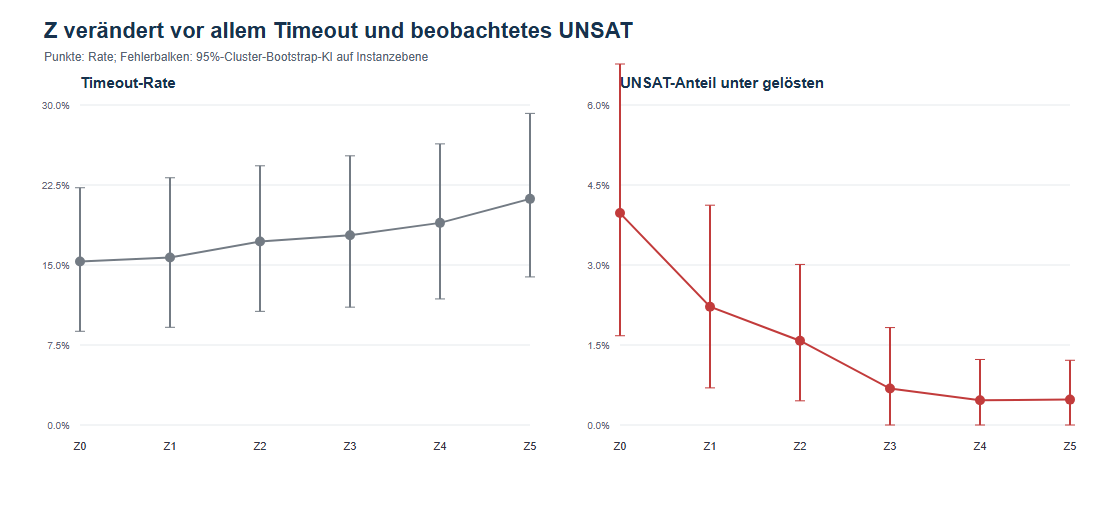
\includegraphics[width=\textwidth]{gfx/analysis_singleton_z/st-z-statusraten.png}
    \caption[Statusraten nach Z-Level]{Empirische Timeout-Rate (links) und
    Anteil beobachteter UNSAT-Ergebnisse unter den gelösten Anfragen
    (rechts) in Abhängigkeit vom \(Z\)-Level. Die Punkte zeigen die
    beobachteten Raten; die Fehlerbalken sind 95\%-Perzentilintervalle eines
    Cluster-Bootstraps mit 4000 Ziehungen vollständiger AF-Instanzen
    (Seed 42). Je Level waren 535 Anfragen vorgesehen; fünf
    Übersetzungsfehler wurden aus den jeweiligen Nennern ausgeschlossen.}
    \label{fig:empirical-stable-z-rates}
\end{figure}

Die gepaarten Kontraste in
Tabelle~\ref{tab:empirical-stable-z-timeout-rd} zeigen einen mit dem Level
zunehmenden Timeout-Unterschied. Für den Hauptkontrast \(Z_5-Z_0\) beträgt
die Risikodifferenz \(5{,}82\) Prozentpunkte
\((95\,\%\text{-KI }[1{,}72;9{,}91],\ p=0{,}0058)\). Der Anstieg ist somit
nicht nur eine Folge unterschiedlicher Instanzzusammensetzungen zwischen
den Leveln, denn jeweils dasselbe Paar wird verglichen. Dass die einzelnen
Kontraste erst ab \(Z_4\) die Schwelle \(p<0{,}05\) unterschreiten, belegt
wegen der explorativen Mehrfachvergleiche keinen scharfen Schwellenwert bei
\(Z_4\).

\begin{table}[H]
    \centering
    \caption[Gepaarte Timeout-Kontraste]{Gepaarte Timeout-Risikodifferenzen
    gegenüber \(Z_0\). Die Effekte sind in Prozentpunkten angegeben.
    Berichtet werden CR1-korrigierte, nach AF geclusterte
    95\%-Konfidenzintervalle und zweiseitige
    Wald-\(p\)-Werte mit \(t_{106}\)-Referenzverteilung. \(N_k\) zählt die
    auf beiden Endpunkten erfolgreich übersetzten Paare.}
    \label{tab:empirical-stable-z-timeout-rd}
    \begin{tabular}{crrrr}
        \toprule
        Kontrast & \(N_k\) & Risikodifferenz & 95\%-KI & \(p\) \\
        \midrule
        \(Z_1-Z_0\) & 535 & \(+0{,}37\) & \([-1{,}29;2{,}04]\) & \(0{,}6568\) \\
        \(Z_2-Z_0\) & 535 & \(+1{,}87\) & \([-0{,}74;4{,}48]\) & \(0{,}1583\) \\
        \(Z_3-Z_0\) & 534 & \(+2{,}43\) & \([-0{,}24;5{,}11]\) & \(0{,}0740\) \\
        \(Z_4-Z_0\) & 533 & \(+3{,}56\) & \([0{,}27;6{,}86]\)  & \(0{,}0341\) \\
        \(Z_5-Z_0\) & 533 & \(+5{,}82\) & \([1{,}72;9{,}91]\)  & \(0{,}0058\) \\
        \bottomrule
    \end{tabular}
\end{table}

Auch im adjustierten Logitmodell ist der Levelkoeffizient positiv. Für den
Schritt von \(Z_k\) zu \(Z_{k+1}\) beträgt die Timeout-Odds-Ratio
\(1{,}110\); unadjustiert ergibt sich \(1{,}081\):
\begin{align*}
    \mathrm{OR}_{\mathrm{adj}}
        &=1{,}110,
        &95\,\%\text{-KI}&=[1{,}028;1{,}198],
        &p&=0{,}0078,\\
    \mathrm{OR}_{\mathrm{unadj}}
        &=1{,}081,
        &95\,\%\text{-KI}&=[1{,}021;1{,}145],
        &p&=0{,}0078.
\end{align*}
Die adjustierte Odds steigt dem Modell zufolge somit pro Level um ungefähr
\(11\,\%\). Dies ist weder mit einer Zunahme der Timeout-Wahrscheinlichkeit
um \(11\,\%\) gleichzusetzen noch als kausaler Effekt zu verstehen.

Als ergänzende nichtparametrische Omnibusanalyse wurde auf den 531 über
alle sechs Level vollständig übersetzten Paaren der Cochran-\(Q\)-Test
berechnet:
\[
    Q=81{,}85,\qquad \mathrm{df}=5,\qquad
    p=3{,}45\cdot10^{-16}.
\]
Er ist die
Erweiterung des McNemar-Tests auf mehr als zwei verbundene binäre
Bedingungen und prüft ohne lineare Trendannahme, ob die marginalen
Timeout-Wahrscheinlichkeiten auf allen sechs Leveln gleich sind. Der Test
liefert weder Richtung noch Effektgröße. Zudem behandelt seine Standardform
die 531 Paare als unabhängige Blöcke und bildet die zusätzliche Gruppierung
von fünf Paaren je AF nicht ab. Er dient daher nur als ergänzende Evidenz;
die Schlussfolgerung stützt sich primär auf die AF-geclusterten
Risikodifferenzen.

Auch eine paarstratifizierte konditionale Logitregression wurde als
Sensitivitätsanalyse gerechnet. Die Konditionierung entfernt den
paarspezifischen Interzept und kontrolliert damit alle über die Level
konstanten Merkmale des AFs und des Paars; die Standardfehler werden
zusätzlich nach AF geclustert. Die bedingte Odds Ratio pro Level beträgt
\[
    \mathrm{OR}_{\mathrm{cond}}=3{,}74,\qquad
    95\,\%\text{-KI}=[1{,}04;13{,}47],\qquad p=0{,}045.
\]
Der
Schätzer wird allerdings ausschließlich von den 36 bezüglich TIMEOUT
variablen Paaren aus zehn AFs bestimmt. Wegen der geringen Zahl informativer
Cluster und des breiten Intervalls wird er nicht als populationsweiter
Haupteffekt, sondern lediglich als Robustheitsbefund interpretiert.

Für beobachtete UNSAT-Abschlüsse ergibt der gepaarte Hauptkontrast
\(Z_5-Z_0\) eine Risikodifferenz von \(-3{,}00\) Prozentpunkten. Die
SAT-Differenz von \(-2{,}81\) Prozentpunkten ist dagegen nicht eindeutig
von null verschieden:
\begin{align*}
    \widehat{\Delta}^{\mathrm{UNSAT}}_5
        &=-3{,}00,
        &95\,\%\text{-KI}&=[-5{,}17;-0{,}84],
        &p&=0{,}0071,\\
    \widehat{\Delta}^{\mathrm{SAT}}_5
        &=-2{,}81,
        &95\,\%\text{-KI}&=[-7{,}12;1{,}49],
        &p&=0{,}198.
\end{align*}
Weil
TIMEOUTs den logischen Ausgang verdecken, belegt der erste Befund nur einen
Rückgang der beobachteten UNSAT-Abschlüsse, nicht einen Rückgang der
tatsächlichen UNSAT-Wahrscheinlichkeit.

Die Übergangsmatrix in
Abbildung~\ref{fig:empirical-stable-z-transitions} verdeutlicht, dass
instanz- und paarspezifische Härte trotz dieses aggregierten Effekts
dominiert. Insgesamt zeigen 482 der 535 Paare
\((90{,}09\,\%)\) über alle erfolgreich übersetzten Level nur einen
Zielstatus. Von den 113 TIMEOUTs auf \(Z_5\) waren 81 bereits auf \(Z_0\)
TIMEOUTs; 32 kamen neu hinzu. Umgekehrt wurde nur ein TIMEOUT von \(Z_0\)
auf \(Z_5\) als SAT gelöst. Größere \(Z\) wirken damit vor allem als
zusätzlicher Belastungsfaktor für eine begrenzte Teilmenge anfälliger Paare.

\begin{figure}[H]
    \centering
    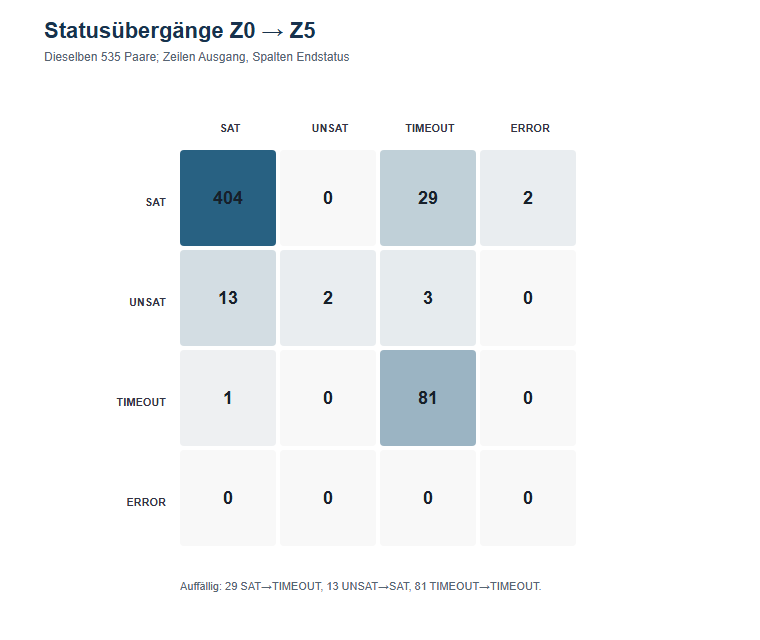
\includegraphics[width=0.82\textwidth]{gfx/analysis_singleton_z/st-z-statusuebergaenge.png}
    \caption[Statusübergänge von Z0 zu Z5]{Übergangsmatrix der Ergebnisse
    derselben 535 Paare zwischen \(Z_0\) (Zeilen) und \(Z_5\) (Spalten).
    Angegeben sind absolute Häufigkeiten; Übersetzungsfehler werden als
    eigene technische Kategorie ausgewiesen. Die Hauptdiagonale beschreibt
    persistente Ergebnisse, die übrigen Zellen Änderungen des beobachteten
    Status.}
    \label{fig:empirical-stable-z-transitions}
\end{figure}

\subsection{Familienabhängigkeit des Z-Effekts}
\label{subsec:empirical-stable-z-families}

Der aggregierte Trend gilt nicht gleichermaßen für alle Instanzfamilien.
Wie Abbildung~\ref{fig:empirical-stable-z-families} zeigt, steigt die
Timeout-Rate der Barabási--Albert-Instanzen von \(0\,\%\) auf \(20\,\%\);
der Anstieg setzt erst auf \(Z_3\) ein und verstärkt sich auf den beiden
größten Leveln. Bei Planning2AF steigt die Rate bereits auf \(Z_1\) auf
\(13{,}3\,\%\) und erreicht ab \(Z_2\) ein Plateau von \(33{,}3\,\%\). Die
gepaarte Risikodifferenz \(Z_5-Z_0\) beträgt für Barabási--Albert
\(20{,}0\) Prozentpunkte. Für Planning2AF liegt die Punktschätzung bei
\(33{,}3\) Prozentpunkten, das Intervall ist aufgrund von nur sechs AFs
jedoch sehr weit:
\begin{align*}
    \widehat{\Delta}^{\mathrm{TO}}_{5,\mathrm{BA}}
        &=20{,}0,
        &95\,\%\text{-KI}&=[3{,}65;36{,}35],
        &p&=0{,}019,\\
    \widehat{\Delta}^{\mathrm{TO}}_{5,\mathrm{Planning}}
        &=33{,}3,
        &95\,\%\text{-KI}&=[-20{,}86;87{,}53],
        &p&=0{,}175.
\end{align*}

Bei Erdős--Rényi schwankt die Timeout-Rate ohne gerichteten Trend zwischen
\(25\,\%\) und \(28\,\%\), beim Stable-Generator bleibt sie auf allen Leveln
bei \(40\,\%\) und bei Watts--Strogatz bei \(15\,\%\). ABA2AF und der
SCC-Generator weisen keine TIMEOUTs auf. Die aggregierte Zunahme wird somit
vor allem von Barabási--Albert und Planning2AF getragen; die Aussage,
größere \(Z\) erschwerten jede Instanz in gleicher Weise, wäre durch die
Daten nicht gedeckt.

\begin{figure}[H]
    \centering
    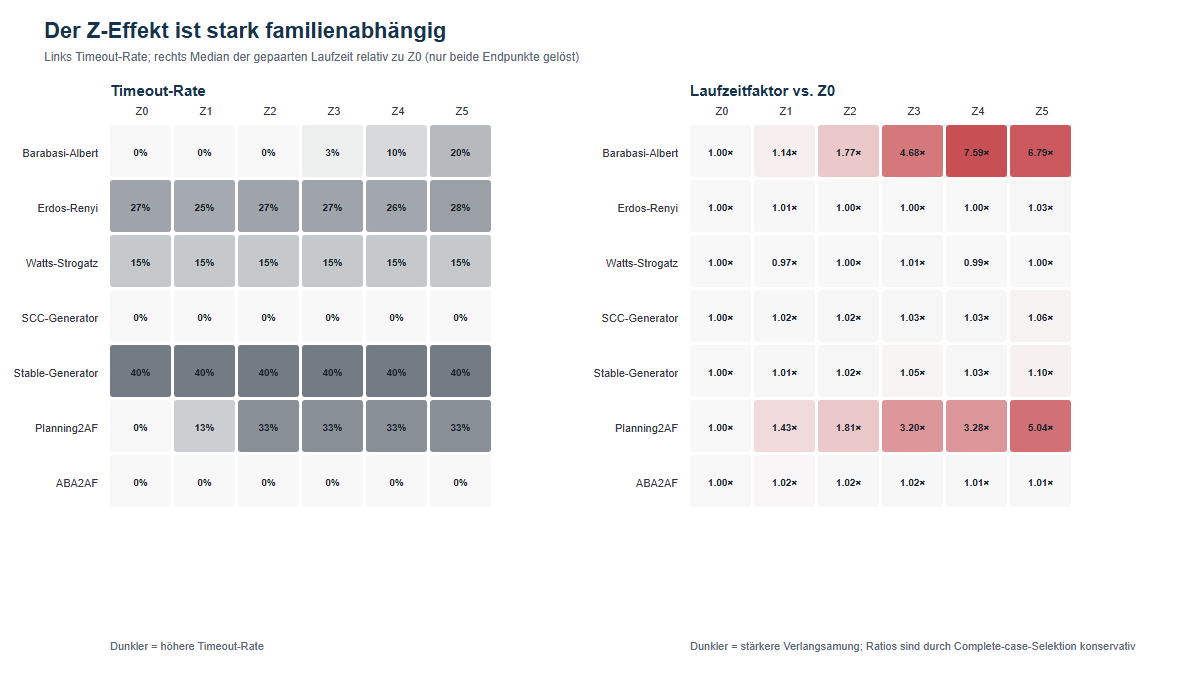
\includegraphics[width=\textwidth]{gfx/analysis_singleton_z/st-z-familien.png}
    \caption[Familienabhängige Effekte der Z-Größe]{Timeout-Raten (links)
    und Median der paarweisen Laufzeitfaktoren relativ zu \(Z_0\) (rechts),
    getrennt nach Instanzfamilie. Für die Laufzeitfaktoren wurden nur Paare
    berücksichtigt, die sowohl auf \(Z_0\) als auch auf dem jeweiligen
    Vergleichslevel gelöst wurden. Neu entstehende TIMEOUTs gehen deshalb
    nicht in die Laufzeitquotienten ein; diese Complete-Case-Auswertung ist
    entsprechend selektiv zu interpretieren.}
    \label{fig:empirical-stable-z-families}
\end{figure}

Auch bei den gelösten Endpunkten konzentriert sich die Verlangsamung auf
diese beiden Familien. Der Median des paarweisen Laufzeitquotienten
\(t(Z_5)/t(Z_0)\) beträgt für Barabási--Albert \(6{,}79\) und für
Planning2AF \(5{,}04\). Für die übrigen Familien liegt er zwischen
\(1{,}00\) und \(1{,}10\). Diese Quotienten unterschätzen den gesamten
Leistungseffekt, weil gerade jene Läufe fehlen, die auf dem größeren Level
neu in einen TIMEOUT wechseln.

\subsection{Solverleistung und QBF-Kodierungsgröße}
\label{subsec:empirical-stable-z-runtime}

Um die Rechtszensierung der Laufzeiten nicht durch eine Auswertung nur der
gelösten Fälle auszublenden, zeigt
Abbildung~\ref{fig:empirical-stable-z-performance} Performanceprofile mit
einem festen Nenner von 535 Anfragen je Level. Der Anteil innerhalb von
\(0{,}1\) Sekunden gelöster Anfragen sinkt von \(44{,}7\,\%\) auf
\(28{,}4\,\%\), innerhalb einer Sekunde von \(57{,}0\,\%\) auf
\(45{,}2\,\%\) und innerhalb von 100 Sekunden von \(81{,}3\,\%\) auf
\(74{,}2\,\%\). Die zum Lösen von \(50\,\%\) aller Anfragen benötigte Zeit
steigt von \(0{,}198\) auf \(1{,}482\) Sekunden. Größere
Konditionierungsmengen verschieben damit nicht nur die Timeout-Rate, sondern
reduzieren bereits bei deutlich kleineren Zeitbudgets den gelösten Anteil.

\begin{figure}[H]
    \centering
    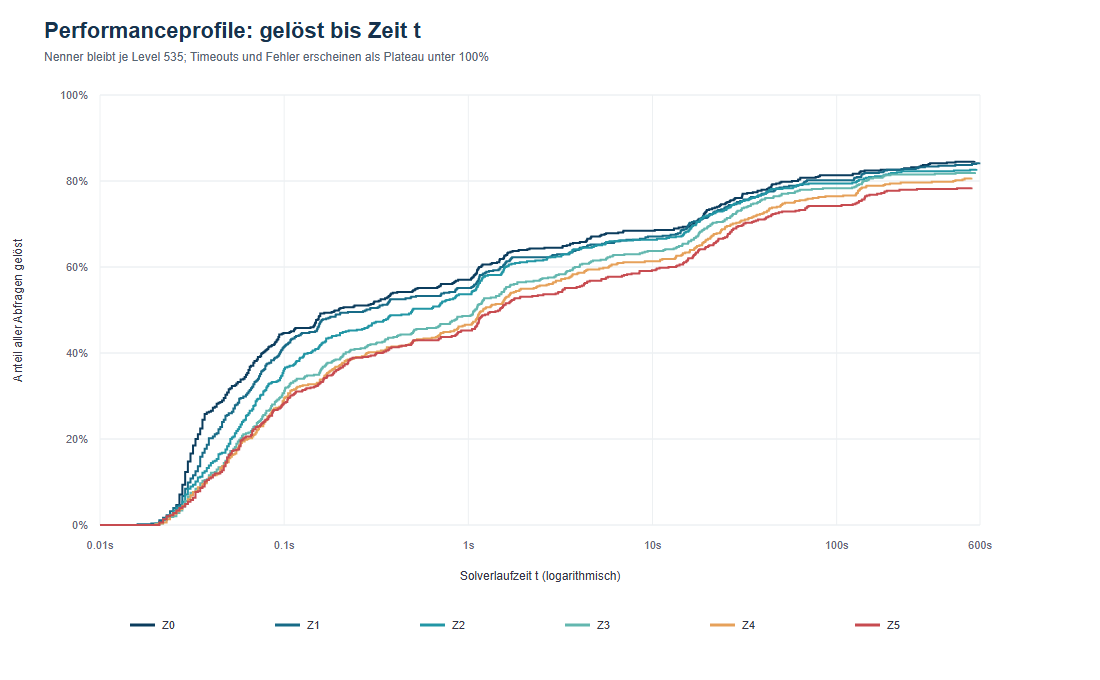
\includegraphics[width=\textwidth]{gfx/analysis_singleton_z/st-z-performanceprofil.png}
    \caption[Performanceprofile nach Z-Level]{Empirische
    Performanceprofile der sechs \(Z\)-Level. Dargestellt ist für jedes
    Zeitbudget \(t\) der Anteil der je Level 535 vorgesehenen Anfragen, die
    bis \(t\) gelöst wurden; die Zeitachse ist logarithmisch. TIMEOUTs bei
    600 Sekunden und Übersetzungsfehler verbleiben im Nenner und führen zu
    Plateaus unter \(100\,\%\). Dies vermeidet die optimistische Selektion
    einer Laufzeitverteilung ausschließlich über gelöste Fälle.}
    \label{fig:empirical-stable-z-performance}
\end{figure}

Der Anstieg der Solverhärte ist nicht allein durch eine proportional
vergleichbare Vergrößerung der Kodierung erklärbar. Für alle 3205
erfolgreichen Übersetzungen gelten exakt
\begin{equation}
    \#\mathrm{Gatter}=12|A|+6|Z|+16,
    \qquad
    \#\mathrm{Variablen}=3|A|.
    \label{eq:empirical-stable-qbf-size}
\end{equation}
Bei gegebenem \(A\) ist die Gatterzahl damit deterministisch an \( |Z| \)
gekoppelt und kann nicht als davon unabhängiger Prädiktor interpretiert
werden.
Zwischen \(Z_0\) und \(Z_5\) steigt die Gatterzahl im Median um
\(9{,}9\,\%\), die QBF-Dateigröße um \(6{,}5\,\%\) und die
Übersetzungszeit um \(1{,}0\,\%\). Dem stehen die Laufzeitfaktoren von
\(6{,}79\) beziehungsweise \(5{,}04\) in den beiden besonders betroffenen
Familien gegenüber
(Abbildung~\ref{fig:empirical-stable-z-qbf-overhead}). Dieser Kontrast
spricht gegen eine Erklärung ausschließlich durch Datei- oder
Übersetzungsgröße und deutet auf eine strukturabhängige Solverhärte hin;
aus der beobachtenden Auswertung folgt jedoch kein kausaler Mechanismus.

\begin{figure}[H]
    \centering
    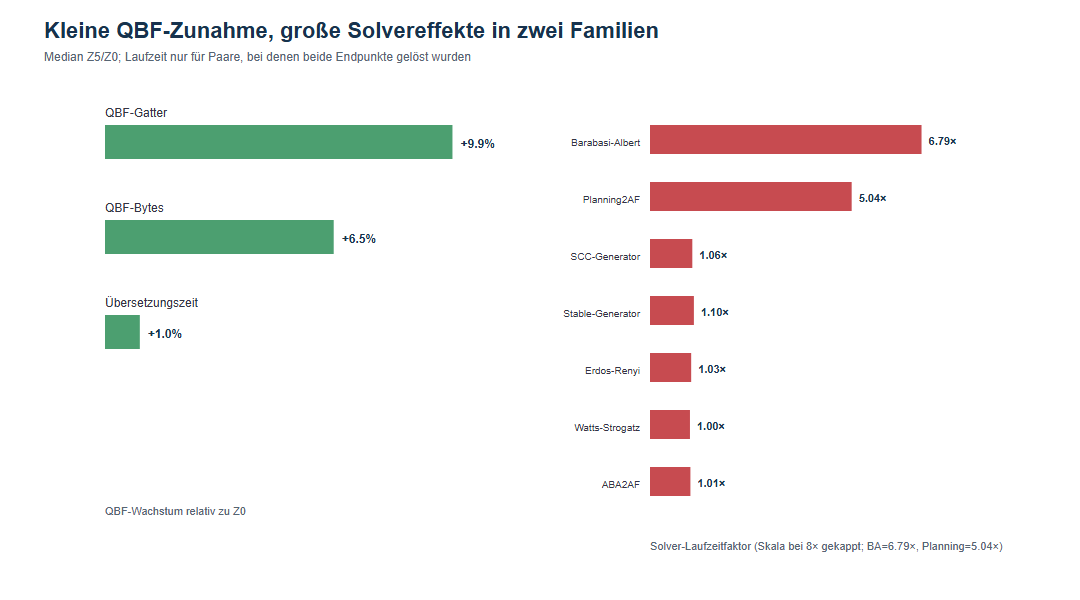
\includegraphics[width=\textwidth]{gfx/analysis_singleton_z/st-z-qbf-overhead.png}
    \caption[QBF-Zuwachs und Solverlaufzeit]{Relative Änderung von \(Z_5\)
    gegenüber \(Z_0\). Links sind die Medianänderungen der QBF-Gatterzahl,
    QBF-Dateigröße und Übersetzungszeit dargestellt; rechts die
    familienweisen Mediane der paarweisen Solverlaufzeitquotienten. Letztere
    beruhen nur auf an beiden Endpunkten gelösten Paaren. Der moderate
    Kodierungszuwachs steht den deutlich höheren Laufzeitfaktoren in
    Barabási--Albert- und Planning2AF-Instanzen gegenüber.}
    \label{fig:empirical-stable-z-qbf-overhead}
\end{figure}

Für die statistische Modellierung wird deshalb \(k\) als primärer
Größenindikator verwendet. Das absolute \( |Z| \) ist
konstruktionsbedingt mit \(n\) gekoppelt. Ein unadjustiertes Logitmodell
ergibt zwar pro zehn zusätzliche Elemente in \(Z\) eine Timeout-Odds-Ratio
von \(1{,}204\) \((95\,\%\text{-KI }[1{,}130;1{,}282])\). Nach
Adjustierung für \(\log n\) und \(\log |R|\) reduziert sie sich jedoch auf
\(1{,}030\) \((95\,\%\text{-KI }[0{,}987;1{,}075],\ p=0{,}167)\).
Die rohe Assoziation mit absolutem \( |Z| \) vermischt somit in erheblichem
Maß den Z-Effekt mit der AF-Größe. Dass das adjustierte Intervall den Wert
eins enthält, beweist umgekehrt nicht die Abwesenheit eines absoluten
Größeneffekts, da die Aussage von der spezifizierten funktionalen Form
abhängt.

\subsection{Einordnung und Einschränkungen}
\label{subsec:empirical-stable-z-limitations}

Insgesamt zeigen die Daten einen moderaten, statistisch nachvollziehbaren
Anstieg des Timeout-Risikos bei größeren Konditionierungsmengen. Zwischen
\(Z_0\) und \(Z_5\) erhöht sich die gepaarte Timeout-Rate um \(5{,}82\)
Prozentpunkte, zugleich verschlechtern sich die Performanceprofile schon
bei kurzen Zeitbudgets. Der Effekt ist jedoch stark heterogen: Er wird
hauptsächlich von Barabási--Albert- und Planning2AF-Instanzen getragen,
während in mehreren Familien die Timeout-Rate konstant bleibt. Der
Rückgang beobachteter UNSAT-Abschlüsse ist wegen der zunehmenden
Rechtszensierung nicht als Nachweis häufiger auftretender semantischer
Unabhängigkeit zu verstehen.

Die Interpretation unterliegt vier wesentlichen Einschränkungen. Erstens
sind die \(Z_k\) nicht geschachtelt und pro Größe liegt nur eine zufällige
Ziehung vor; der reine Größeneffekt ist daher nicht von der konkreten
Zusammensetzung der Menge trennbar. Zweitens können neu auftretende
TIMEOUTs eine selektive Complete-Case-Laufzeitanalyse verzerren, weshalb die
Performanceprofile als belastbarere Gesamtdarstellung herangezogen werden.
Drittens stammen die 107 AFs aus einer Benchmarkauswahl und bilden keine
Zufallsstichprobe aller AFs; die Konfidenzintervalle setzen unabhängige
AF-Cluster voraus und rechtfertigen keine uneingeschränkte Generalisierung.
Viertens sind die zahlreichen Detailvergleiche explorativ und nicht für
Multiplizität korrigiert. Die robuste Kernaussage beschränkt sich deshalb
auf den aggregierten, AF-geclusterten Anstieg des Timeout-Risikos und seine
ausgeprägte Familienabhängigkeit.